%-------------------------------------------------------------------------------
%-------------------------------------------------------------------------------
%-------------------------------------------------------------------------------
\chapter{Logique}
%-------------------------------------------------------------------------------
%-------------------------------------------------------------------------------
\thispagestyle{empty}
%-------------------------------------------------------------------------------
%-------------------------------------------------------------------------------
%--------------------------------------------------------------------------
%--------------------------------------------------------------------------
%--------------------------------------------------------------------------
\section{Présentation du problème}
%--------------------------------------------------------------------------
%--------------------------------------------------------------------------
On se propose ici de gérer les propositions logiques de manière élémentaire et d'étudier le problème de la satisfiabilité.

Quelques applications ludiques sont proposées en conclusion.

\begin{itemize}
  \item Les propositions booléennes seront codées à l'aide du type

\begin{lstlisting}
type propBool =  X of int
                |Non of propBool
                |Ou of propBool*propBool
                |Et of propBool*propBool;;
\end{lstlisting}


\item \type{X k} désignera une variable booléenne indexée par $k$ que l'on notera $x_k$.

Nous n'utiliserons que des variables indexées par des entiers supérieurs ou égaux à 1.

\item Par exemple la proposition $x_1 \lor \bigl(\lnot (x_2 \lor \lnot x_1) \land x_3\bigr)$ sera comprise par

\begin{lstlisting}
let p_ex = Ou (X 1, Et (Non (Ou (X 2, Non (X 1))), X 3));;
\end{lstlisting}

\item Si les variables booléennes ont un indice majoré par $n$ on représentera une valuation par un tableau de booléens de taille $n$, \type{val}. La valeur attribuée à \type{X k} sera \type{val.(k-1)}. 
\end{itemize}

%--------------------------------------------------------------------------
%--------------------------------------------------------------------------
%--------------------------------------------------------------------------
\section{Outils}
%--------------------------------------------------------------------------
%--------------------------------------------------------------------------
%--------------------------------------------------------------------------
On veut pouvoir écrire les expression booléennes de manière plus lisible. 

Par exemple, la formule \type{p\_ex} pourra être imprimée sous la forme
\begin{lstlisting}
x1 V (!(x2 V !x1) & x3))
\end{lstlisting}
%--------------------------------------------------------------------------
%--------------------------------------------------------------------------
\begin{Exercise}\it 
Écrire une fonction \type{montrer} qui permet cette visualisation.

La concaténation de chaînes se fait avec \type{str1\^{}str2} 

et on convertit un entier en chaîne par \type{string\_of\_int}.
\end{Exercise}
%--------------------------------------------------------------------------
\begin{Answer}
\begin{lstlisting}
let symOu = " V ";; 
let symEt = " & ";; 
let symNon = "!";;
let rec montrer X =
  match X with
  |Var(k) -> "x"^(string_of_int k)
  |Non(q) -> symNon^(montrer q)
  |Ou(q,r) -> "("^(montrer q)^symOu^(montrer r)^")"
  |Et(q,r) -> "("^(montrer q)^symEt^(montrer r)^")";;
\end{lstlisting}
\end{Answer}
%--------------------------------------------------------------------------
%--------------------------------------------------------------------------
\begin{Exercise}\it
Écrire une fonction \type{multiOu} de type \type{propBool List -> propBool} qui, en recevant une liste non vide de propositions logiques \type{[P1; P2; ...; Pn]}, renvoie la disjonction des $P_i$.

Écrire de même une fonction \type{multiEt}
\end{Exercise}
%--------------------------------------------------------------------------
\begin{Answer}
\begin{lstlisting}
let rec multiOu listeX =
  match listeX with
  |[] -> failwith "La liste est vide"
  |[p] -> p
  |t::q -> Ou(t, multiOu q);;
  
let rec multiEt listeX =
  match listeX with
  |[] -> failwith "La liste est vide"
  |[p] -> p
  |t::q -> Et(t, multiEt q);;
\end{lstlisting}
\end{Answer}
%--------------------------------------------------------------------------
\newpage
%--------------------------------------------------------------------------
\begin{Exercise}\it
Écrire une fonction \type{implique} qui calcule une proposition logiquement équivalente à $\type{P1} \Rightarrow \type{P1}$ à partir de deux propositions \type{P1} et \type{P2}.

Écrire de même des fonction \type{equivaut} et \type{ouExclusif}.
\end{Exercise}
%--------------------------------------------------------------------------
\begin{Answer}
\begin{lstlisting}
let implique X q = Ou(Non p, q);;

let equivaut X q = Ou(Et(p, q), Et(Non p, Non q));;

let ouExclusif X q = Ou(Et(p, Non q), Et(Non p, q));;
\end{lstlisting}
\end{Answer}
%--------------------------------------------------------------------------
%--------------------------------------------------------------------------
\begin{Exercise}\it
Écrire une fonction (récursive) \type{uneSeule} qui prend pour argument une liste de propositions et calcule  une proposition qui est vraie si et seulement s’il y a exactement une des propositions de la liste qui est vraie.
\end{Exercise}
%--------------------------------------------------------------------------
\begin{Answer}
\begin{lstlisting}
let rec uneSeule listeX =
  match listeX with
  |[] -> failwith "La liste est vide"
  |[p] -> p
  |t::q -> Ou(Et(Non t, uneSeule q), Et(t, Non (multiOu q)));;
\end{lstlisting}
\end{Answer}
%--------------------------------------------------------------------------
%--------------------------------------------------------------------------
%--------------------------------------------------------------------------
\section{Évaluation}
%--------------------------------------------------------------------------
%--------------------------------------------------------------------------
\begin{Exercise}\it
Écrire une fonction \type{eval} qui renvoie la valeur booléenne d'une proposition booléenne pour une valuation. Par exemple
\begin{lstlisting}
eval p_ex [|true; false; true|];;
#- : bool = true
\end{lstlisting}
\end{Exercise}
%--------------------------------------------------------------------------
\begin{Answer}
\begin{lstlisting}
let rec eval X t =
  match X with
  |Var(k) -> t.(k-1)
  |Non(q) -> not (eval q t)
  |Ou(q,r) -> (eval q t) || (eval r t)
  |Et(q,r) -> (eval q t) && (eval r t);;
\end{lstlisting}
\newpage
\end{Answer}
%--------------------------------------------------------------------------
%--------------------------------------------------------------------------
\begin{Exercise}\it
Écrire une fonction \type{indiceMax} qui renvoie l’indice de variable maximal rencontré dans une proposition logique.
\end{Exercise}
%--------------------------------------------------------------------------
\begin{Answer}
\begin{lstlisting}
let rec indiceMax X =
  match X with
  |Var(k) -> k
  |Non(q) -> indiceMax q
  |Ou(q,r) -> max (indiceMax q) (indiceMax r)
  |Et(q,r) -> max (indiceMax q) (indiceMax r);;
\end{lstlisting}
\end{Answer}
%--------------------------------------------------------------------------
%--------------------------------------------------------------------------
\medskip


Pour pouvoir décrire toutes les valuations nous allons utiliser une fonction \type{incremente} qui modifie un tableau de booléens (sans renvoyer sa valeur) et qui renvoie \type{true} sauf quand le tableau n'est pas incrémentable. On suit l'algorithme qui correspond à l'incrémentation d'un entier exprimé en base 2 :
\begin{itemize}
\item on modifie les indices les plus petits de \type{true} à \type{false}
\item s'il existe, le premier \type{false} est modifé en \type{true} et la fonction renvoie \type{true}
\item s'il n'y avait que des \type{true} la fonction renvoie \type{false} pour signifier que toutes les valuations ont été parcourues.
\end{itemize}
%--------------------------------------------------------------------------
\begin{Exercise}\it
Écrire la fonction \type{incremente}.
\end{Exercise}
%--------------------------------------------------------------------------
\begin{Answer}
\begin{lstlisting}
let incremente t =
  let rec aux_inc pos =
    if pos = Array.length t
    then false
    else if t.(pos)
         then (t.(pos) <- false;  aux_inc (pos+1))
         else (t.(pos) <- true; true)
  in aux_inc 0;;       
\end{lstlisting}
\end{Answer}
%--------------------------------------------------------------------------
%--------------------------------------------------------------------------
\begin{Exercise}\it 
Écrire une fonction \type{possibles} qui renvoie la liste des tableaux satisfaisant une proposition logique. 

On copiera les tableaux à l’aide de la fonction \type{Array.copy}.
\end{Exercise}
%--------------------------------------------------------------------------
\begin{Answer}
\begin{lstlisting}
let possibles X =
  let n = indiceMax X in
  let t = Array.make n false in
  let sol = ref [] in
  if eval X t then sol := t::(!sol);
  while (incremente t)
  do if eval X t
     then sol := (Array.copy)::(!sol) done;
  !sol;;
\end{lstlisting}
\end{Answer}
%--------------------------------------------------------------------------
%--------------------------------------------------------------------------
\begin{Exercise}\it 
Écrire deux fonctions \type{satisfiable} et \type{tautologie} qui déterminent respectivement si une proposition logique est satisfiable et si c’est une tautologie.
\end{Exercise}
%--------------------------------------------------------------------------
\begin{Answer}
\begin{lstlisting}
let satisfiable X = possibles p <> [];;

let tautologie X = not (satisfiable (Non(p)));;
\end{lstlisting}
\end{Answer}
%--------------------------------------------------------------------------
%--------------------------------------------------------------------------
\begin{Exercise}\it
Vérifier que les propositions suivantes sont des tautologies.
\begin{enumerate}
  \item $\lnot \lnot x_1 \Leftrightarrow x_1$
  \item $(x_1 \Rightarrow x_2)\Leftrightarrow(\lnot x_2 \Rightarrow \lnot x_1)$
  \item $(x_1 \Rightarrow x_2) \land (x_2 \Rightarrow x_3) \Rightarrow (x_1 \Rightarrow x_3)$
\end{enumerate}
\end{Exercise}
%--------------------------------------------------------------------------
\begin{Answer}
\begin{lstlisting}
let x1 = X 1;;
let x2 = X 2;;
let x3 = X 3;;

let p1 = implique (Non(Non x1)) x1;;
let p2 = equivaut (implique x1 x2) 
                  (implique (Non x2) (Non x1));;
let p3 = implique (Et (implique x1 x2,implique x2 x3)) 
                  (implique x1 x3);;

tautologie p1;;
tautologie p2;;
tautologie p3;;
\end{lstlisting}
\newpage
\end{Answer}
%--------------------------------------------------------------------------
%--------------------------------------------------------------------------
\newpage
%--------------------------------------------------------------------------
\section{Exemples}
% %--------------------------------------------------------------------------
% %--------------------------------------------------------------------------
% \subsection{Les dahuts}
% %--------------------------------------------------------------------------
% %--------------------------------------------------------------------------
% \begin{wrapfigure}{l}{0.32\textwidth}
% \vskiX -3mm
% 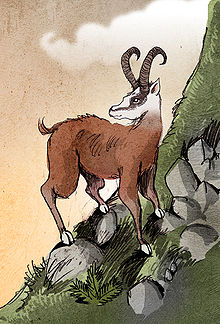
\includegraphics[width=0.30\textwidth]{dahut}
% \vskiX -2cm 
% \end{wrapfigure}
% Le dahut est une espèce très rare de bouquetin qui a la particularité d'avoir les deux pattes d'un coté plus courtes que les autres. Il vit donc dans la montagne en ayant toujours le sommet du coté de ses pattes courtes.
%  Un dahut est appelé de dextrogyre ou lévogyre selon les cas.
 
%  Ils ont d'autres particularités :
 
%  \begin{itemize}
% \item Tout dahut non lévogyre a des rayures noires.
% \item Tout dahut a des oreilles blanches ou n'a pas de rayures noires.
% \item Les dahuts qui vivent dans les forêts ne mangent pas de mulots.
% \item Un  dahut mange des mulots si et seulement s'il est lévogyre.
% \item Tout  dahut qui a des oreilles blanches est lévogyre et vit dans les forêts.
% \item Tout  dahut lévogyre a des oreilles blanches.
%  \end{itemize}
% %--------------------------------------------------------------------------
% %--------------------------------------------------------------------------
% \begin{Exercise}
% Prouver que les dahuts n'existent pas.
% \end{Exercise}
% %--------------------------------------------------------------------------
% %--------------------------------------------------------------------------
% \subsection{La princesse}
% %--------------------------------------------------------------------------
% %--------------------------------------------------------------------------
% Un chevalier doit partir délivrer des princesses. Arrivé à une intersection, il a le choix entre trois chemins, chacun précédé d'un panneau. Le gardien des lieux lui déclare : ''Parmi ces trois chemins, l'un mène à une princesse, et son panneau dit la vérité. Quant aux deux autres, ils aboutissent
% à une mort certaine. Au moins l'un des panneaux ment.''
% Voici ce qui est écrit à l'entrée de chaque chemin :

% \begin{itemize}
% \item Le deuxième chemin mène à une mort certaine.
% \item Ce chemin mène à une mort certaine.
% \item Le premier chemin mène à une mort certaine.
% \end{itemize}
% %--------------------------------------------------------------------------
% %--------------------------------------------------------------------------
% \begin{Exercise}
% Comment délivrer la princesse ?
% \end{Exercise}
% %--------------------------------------------------------------------------
% \begin{Answer}
% Prendre le premier chemin.
% \end{Answer}
%--------------------------------------------------------------------------
%--------------------------------------------------------------------------
\subsection{Le concours}
%--------------------------------------------------------------------------
%--------------------------------------------------------------------------
Vous êtes admissible à l'Université de Logique Médiévale (ULM) et vous devez passer l'épreuve de logique pratique. Depuis le Hall d'entrée il y a 5 couloirs et vous savez qu'un seul mène à la salle d'examen.

Chaque couloir est indiqué par un panneau et vous savez aussi que le panneau qui mène à votre salle dit la vérité mais que les autres peuvent mentir.

Voici ce que disent les cinq panneaux.

\begin{enumerate}
\item Ce couloir vous mène à l'échec mais pas le quatrième.
\item C’est un chemin de numéro impair qui mène dans la salle.
\item Le deuxième panneau dit la vérité ou le cinquième ment.
\item Ce panneau ment mais pas le premier.
\item Le troisième panneau ment.
\end{enumerate}
%--------------------------------------------------------------------------
%--------------------------------------------------------------------------
\begin{Exercise}\it
Comment arriver à votre salle ?
\end{Exercise}
%--------------------------------------------------------------------------
\begin{Answer}
\begin{lstlisting}
let x1 = X 1;;
let x2 = X 2;;
let x3 = X 3;;
let x4 = X 4;;
let x5 = X 5;;
let p1 = X 6;;
let p2 = X 7;;
let p3 = X 8;;
let p4 = X 9;;
let p5 = X 10;;

let c1 = implique x1 p1;;
let c2 = implique x2 p2;;
let c3 = implique x3 p3;;
let c4 = implique x4 p4;;
let c5 = implique x5 p5;;

let u = uneSeule [x1; x2; x3; x4; x5];;

let e1 = equivaut p1 (Et (Non x1, x4));;
let e2 = equivaut p2 (multiOu [x1; x3; x5]);;
let e3 = equivaut p3 (Ou (p2, Non p5));;
let e4 = equivaut p4 (Et (Non p4, p1));;
let e5 = equivaut p5 (Non p3);;

let p = multiEt [c1; c2; c3; c4; c5; u; e1; e2; e3; e4; e5];; 

possibles jeu1;;
\end{lstlisting}
Prendre le troisième couloir.
\newpage
\end{Answer}
%--------------------------------------------------------------------------
%--------------------------------------------------------------------------
\subsection{Le cadeau}
%--------------------------------------------------------------------------
%--------------------------------------------------------------------------
Vous êtes admis dans l'école de vos rêves ! Pour vous accueillir les camarades de deuxième année vous offrent un Kinder.
Mais il faut le mériter : vous avez devant vous 9 boîtes dont une seule contient l'œuf. De plus chacune a une étiquette et votre parrain vous annonce que la boîte qui contient votre cadeau porte une étiquette qui dit la vérité les autres peuvent mentir.

Voici les énoncés.


\begin{enumerate}
\item C’est une boîte de numéro impair qui contient la récompense
\item Ouvre-moi si tu veux du chocolat.
\item La cinquième étiquette dit la vérité ou la septième ment. Mais la neuvième ment.
\item La première étiquette ment.
\item Parmi la deuxième et la quatrième étiquette, il y en a au moins une qui dit la vérité.
\item La troisième étiquette ment.
\item La première boîte est vide.
\item Je ne dis pas la vérité et la neuvième boîte contient le cadeau.
\item Il ne faut pas croire la sixième étiquette.
\end{enumerate}
%--------------------------------------------------------------------------
%--------------------------------------------------------------------------
\begin{Exercise}\it 
Quelle boîte ouvrez-vous ?
\end{Exercise}
%--------------------------------------------------------------------------
\begin{Answer}
\begin{lstlisting}
let x1 = X 1;;
let x2 = X 2;;
let x3 = X 3;;
let x4 = X 4;;
let x5 = X 5;;
let x6 = X 6;;
let x7 = X 7;;
let x8 = X 8;;
let x9 = X 9;;
let p1 = X 10;;
let p2 = X 11;;
let p3 = X 12;;
let p4 = X 13;;
let p5 = X 14;;
let p6 = X 15;;
let p7 = X 16;;
let p8 = X 17;;
let p9 = X 18;;

let c1 = implique x1 p1;;
let c2 = implique x2 p2;;
let c3 = implique x3 p3;;
let c4 = implique x4 p4;;
let c5 = implique x5 p5;;
let c6 = implique x6 p6;;
let c7 = implique x7 p7;;
let c8 = implique x8 p8;;
let c9 = implique x9 p9;;

let u = uneSeule [x1; x2; x3; x4; x5; x6; x7; x8; x9];;

let e1 = equivaut p1 (multiOu [x1; x3; x5; x7; x9]);;
let e2 = equivaut p2 x2;;
let e3 = equivaut p3 (Et (Ou (p5, Non p7), Non p9));;
let e4 = equivaut p4 (Non p1);;
let e5 = equivaut p5 (Ou (p2, p4));;
let e6 = equivaut p6 (Non p3);;
let e7 = equivaut p7 (Non x1);;
let e8 = equivaut p8 (Et (Non p8, x9));;
let e9 = equivaut p9 (Non p6);;

let jeu3 = multiEt [c1; c2; c3; c4; c5; c6; c7; c8; c9; u; e1; e2; e3; e4; e5; e6; e7; e8; e9];; 

possibles jeu3;;
\end{lstlisting}
La septième.
\end{Answer}
